\documentclass{article}

\usepackage{url}
\usepackage{blindtext}
\usepackage{siunitx} 
\usepackage{graphicx} 
\usepackage{amsmath} 
\usepackage{amsfonts}
\usepackage[margin=0.5in]{geometry}
\usepackage[export]{adjustbox}
\usepackage{wrapfig}
\usepackage{subcaption}
\usepackage{multicol}
\setlength{\columnsep}{1cm}
\usepackage{bm}
\usepackage{pdfpages}
\usepackage{color}
\usepackage[backend=bibtex8, style = numeric]{biblatex}
\addbibresource{project_bib.bib}

\usepackage{newunicodechar}
\newunicodechar{π}{\ensuremath{\pi}}

\setlength\parindent{0pt}

\usepackage{times} % Uncomment to use the Times New Roman font
\newenvironment{Figure}
  {\par\medskip\noindent\minipage{\linewidth}}
  {\endminipage\par\medskip}

%----------------------------------------------------------------------------------------
%	DOCUMENT INFORMATION
%----------------------------------------------------------------------------------------
\begin{document}

\title{ \line(1,0){500} \\ \textbf{Understanding QCD dynamics through pPb collisions at the LHC}  \\ \line(1,0){500}}

\date{\vspace{-5ex}}

\maketitle % Insert the title, author and date

\vspace{1.5cm}

\begin{center}
\begin{tabular}{l l}


\large Author:  Allencris John Rubesh Rajan 

&

\large Supervisor: \large Prof. Ronan McNulty

\end{tabular}
\end{center}

\pagestyle{empty}

\vfill % equivalent to \vspace{\fill}
\clearpage

\pagebreak

\topskip0pt
\vspace*{\fill}
\begin{center}
\Large \textbf{Acknowledgements}
\end{center}

\large 
\vspace*{\fill}



\pagebreak

\begin{center}
\line(1,0){500}

\end{center}
\begin{abstract}

\end{abstract}
\begin{center}

\line(1,0){500}
\end{center}

\vspace{0.5cm}

%----------------------------------------------------------------------------------------
%	SECTION 1
%----------------------------------------------------------------------------------------

\begin{multicols}{2}

\section{Introduction} 


\section{The Weizsäcker-Williams Approximation}

In ultra-peripheral hadron-hadron collisions, the only interaction mechanism available to the hadrons is electromagnetism. Thus, we must use a method originally developed by Enrico Fermi in 1924 to handle collisional problems in a paper entitled "On the Theory of Collisions between Atoms and Elastically Charged Particles".\cite{fermi} He drew parallels between the electromagnetic fields of the charged particles in a given collision problem and the electric fields of pulses of radiation, treating the fields of the charged particle as a flux of virtual photons. This method was then extended by Weiszäcker and Williams a decade later to ultra-relativistic particles. Thus, the method is known as either the equivalent photon approximation or the Weiszäcker-Williams method.
\\\\
As pictured in figure \ref{fig1}, the electric fields vectors of a relativistic charged particle point radially outward with the magnetic fields circling it. Through a fourier transform, these fields can be replaced by an equivalent pulse of radiation. We shall give the derivation here, following the approach given by Jackson. \cite{jackson}
\\\\
As in any given collision, we shall look at this in terms of the "incident particle" and the "struck system". In our derivation, we shall consider the incident particle to be an ion of charge Z and the struck system to be a proton. Furthermore, as we are interested in ultra-peripheral collisions, we only consider values for the impact parameter exceeding the sum of the radii of the ion and proton: $b > R_{I} + R{p}$ where the radii are given by \begin{equation}
R = R_{0} A^{\frac{1}{3}}
\end{equation}
$R_{0}$ is typically taken to be $1.25 \unit{\femto \meter}$. \cite{r0} The spectrum of equivalent radiation from the ion when it has velocity $v \approx c$, passing the proton at an impact parameter $b$ can be found by performing a fourier transform of the electric fields transverse and longitudinal components of its electric field. To compute the electric field in the lab frame, we shall first consider the problem from the ion's frame $K^{'}$ (see Fig. \ref{fig2}). For the sake of our analysis, we shall consider the two frames to coincide at $t = 0$. As the ion only has a velocity in the positive $(x^{1})$ direction, $(x^{2}) = (x^{2})^{'}= b$ and $(x^{2}) = (x^{2})^{'}= 0$. Now we can very simply write the ion's electric field in the frame its own frame as:

\begin{Figure}
\centering
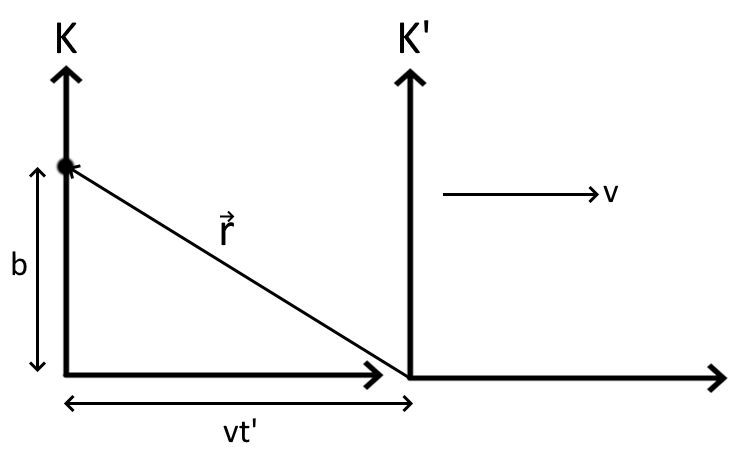
\includegraphics[width=\linewidth]{sr.png}
\captionof{figure}{The incident particle (frame $K^{'}$ travels away from the lab frame $K$ with velocity $v$ in the $x^{1}$ direction.}
\label{fig2}
\end{Figure}

\end{multicols}

\begin{Figure}
\centering
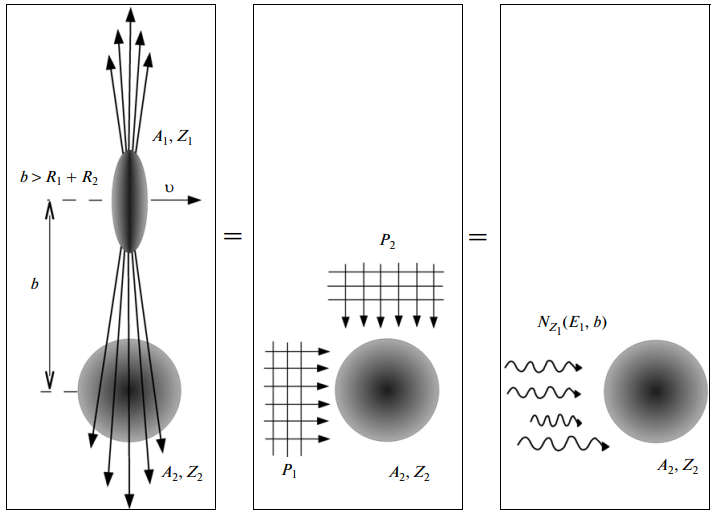
\includegraphics[width=0.8\linewidth]{EPA.png}
\captionof{figure}{In UPCs, charged particles interact through their electromagnetic fields. Through the equivalent photon method, the effect of the electric field of $A1$ can be approximated as the absorption of a flux of equivalent radiation with momenta $P1$ and $P2$ by the $A2$. This results in the spectrum $N_{Z1}(E_{1},b)$. \cite{eepa}}
\label{fig1}
\end{Figure}

\section{Conclusion}





\vspace{1cm}

\pagebreak

\printbibliography



\end{document}
